\chapter{Background}
\label{ch02}
This chapter discusses relevant topics to this thesis and state-of-the-art of anycast measurements. It is started with the concept of DNS (Section \ref{ch02:dns}) and IP anycast (Section \ref{ch02:anycast}). Next, methodologies used for anycast DNS measurements as described in the literature are discussed in Section \ref{ch02:measuring-anycast}. Subsequently, the measurement of catchment areas from control-plane perspective is described in Section \ref{ch02:control-plane}. Then, state-of-the-art of anycast visualization is discussed in Section \ref{ch02:visualization}. Section \ref{ch02:concluding} provides the concluding remarks of this chapter.

\section{DNS}
\label{ch02:dns}
As described in RFC 1034 \cite{rfc1034}, \textit{Domain Name System} (DNS) is a distributed database system that essentially provides mapping between IP address and the corresponding name, and vice versa. The data for the mapping is stored in an inverted-tree-structured distributed database (Figure \ref{fig:dns-tree}), where each node is called \textit{domain}. The topmost level of the hierarchy is called the \textit{root domain}, represented by a single dot ('.'), and becomes the starting point of a query. The next level consists of \textit{top-level domains} (TLDs), \textit{e.g.}, \texttt{.com}, \texttt{.net}, \texttt{.id}, and so on. Each domain becomes the root of  a new \textit{subdomain}. Every domain has a unique name, called \textit{fully-qualified domain name} (FQDN), which is the sequence of labels from the node at the root of the domain to the root domain. Each domain can be divided further into \textit{subdomains}, and responsibility for each subdomain can be delegated to a different organization.

\begin{figure}
	\centering
	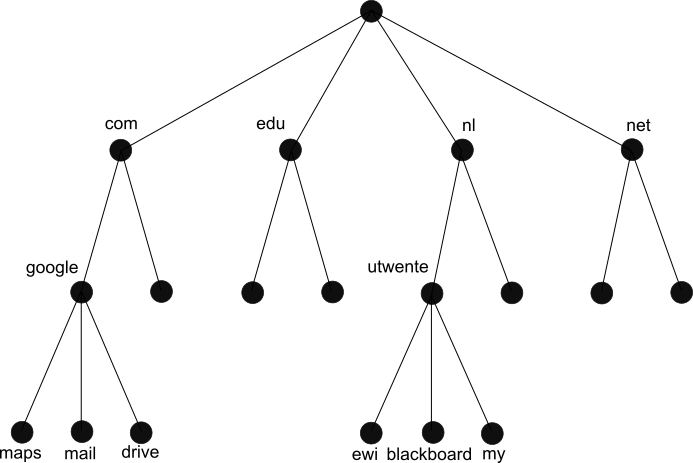
\includegraphics[scale=0.45]{img/dns-tree.png}
	\caption{Example of DNS database tree}
	\label{fig:dns-tree}
\end{figure}

The DNS has three major components \cite{rfc1034}:
\begin{description}
	\setlength{\itemsep}{1pt}
	\setlength{\parskip}{0pt}
	\item[The domain name space and resource records] A domain name \cite{rfc1035} identifies a node, and the goal of domain names is to provide a mechanism for naming resources (re-corded as \textit{resource records}, RRs) in such a way that the names are usable in different hosts, networks, protocol families, and administrative organizations. 
	\item[Nameservers] Nameservers manage two types of data. Firstly, it maintains \textit{zones}, where each zone is the complete database for a particular segment of domain space (called authoritative). Secondly, it keeps \textit{cached data} acquired by local resolvers, and used to improve the performance of query process when non-local data is frequently accessed. Nameservers also have pointers to other name servers that can be used to lead to information from any part of the domain tree. 
	\item[Resolvers] The local agent that accesses	 nameservers due to query requests from clients. It handles a nameserver queries, response interpretation, and returning the information to the requesting clients. 
\end{description}

\textit{Root nameservers}, shortly called \textit{Root Servers}, is the nameservers for root zone. It contains information of the authoritative nameservers for each of TLD zones. Any DNS queries, except for queries in the authoritative list of a nameserver, requires a response from a root server to be answered (and the answer can be cached for some determined time). 

Root Servers role is critical in DNS because they are needed for the first step of DNS translation. Without them, the DNS simply does not work. Considering that DNS becomes one of the fundamental protocol in Internet infrastructure, failure in DNS may results in major broken connectivities. Currently, there are 13 Root Servers in the world (named from \texttt{A} to \texttt{M}) managed by different organizations, with the names in the form of \texttt{<alphabet>.root-servers.net}. The comprehensive information about Root Servers and their distributions around the world are available in \cite{site:root-servers}.

%The TLDs are categorized into two: \textit{gTLDs} and \textit{ccTLDs}. gTLD is \textit{generic}, in the sense that it can be (theoretically) used by anyone and anywhere. Some well-known examples are \texttt{.com}, \texttt{.net}, and \texttt{.org}. ccTLDs are assigned to countries based on ISO 3166\footnote{\url{http://www.iso.org/iso/country_codes}} list of country codes. Examples are \texttt{.nl}, \texttt{.uk}, \texttt{.it}, and \texttt{.id}.

%To identify resource, RR has the following information: \textit{owner}, which is the domain name where the RR is found; \textit{type}, to specifies the type of the resource; \textit{class}, to identify a protocol family; and \textit{TTL} of the RR. Typically, the most used class is \textit{Internet} (\texttt{IN}). Another one is \texttt{CHAOS} (from Chaosnet protocol \cite{chaosnet}), of which now is used for name server instance identification \cite{rfc4892}. Some examples of RR types are \textit{\texttt{A}}, which is used for host-to-IPv4 address record; \textit{\texttt{AAAA}} for host-to-IPv6; \textit{\texttt{PTR}} for host-to-IP address; and \textit{\texttt{MX}} for mail exchange information. Recently, \textit{\texttt{DS}} and \textit{\texttt{DNSKEY}} have also gained popularity with the increasing deployment of DNSSEC \cite{rfc4641}. The complete list of the classes is available at \cite{iana-dnsparam}. 

%In production environment, it is likely that a single IP address of a DNS server is in fact shared by multiple servers. It might be because of load balancing purpose or the use of anycast. RFC 4892 \cite{rfc4892} provides recommendation on how to identify DNS server. It recommends to query a \texttt{TXT} resource record in class 3 (\texttt{CHAOS}) for the domain name \texttt{HOSTNAME.BIND}. The administrator can then configure this by the unique identifier of the responding server.

\section{IP Anycast}
\label{ch02:anycast}

RFC 1546 \cite{rfc1546} describes IP anycast as a technique to share IP address in common among multiple nodes in multiple locations relying on the BGP routing to map clients to anycast nodes (\textit{one-to-any} connection). Figure \ref{fig:anycast} illustrates conceptual anycast. A client (red node)  sends datagrams towards an anycast address, which is assigned to a group of nodes (green ones). The routing scheme on the network will deliver the datagrams towards \textit{one} of the green nodes which satisfies the best-fit requirement (typically the shortest topological distance). Anycast is intended for services where the users are only care about the service delivery, regardless which server provides it. 

\begin{figure}[ht!]
	\centering
	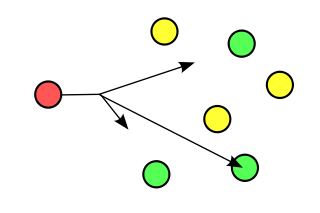
\includegraphics[scale=0.5]{img/anycast.png}
	\caption{Illustration of anycast (copied from \cite{wiki-anycast})}
	\label{fig:anycast}
\end{figure}

There is also another type of anycast, called \textit{application-layer anycast} \cite{631176}. As the name implies, it works at the application layer. In contrast, IP anycast works in network layer. This thesis focuses on IP anycast only. For the rest of this report, \textit{IP anycast} and \textit{anycast} are used interchangeably.

\iffalse
Despite of its simplicity, IP anycast is known to have some notable limitations \cite{631176,ballani2005towards}: 
\begin{description}
	\setlength{\itemsep}{1pt}
	\setlength{\parskip}{0pt}
	\setlength{\parsep}{0pt}
	\item \textbf{Poor scalability}. Deploying IP anycast globally requires an adequate size of address block (\textit{i.e.}, /24) in order to be properly advertised in BGP by its upstream ISP. On the other hand, routes for IP anycast groups cannot be aggregrated, since the routing infrastructure must support one route per IP anycast group. 	
	\item \textbf{Only suitable for connectionless application}. IP anycast forwarding is performed per-datagram basis. Thus, if there is route changes in the network during transmissions, sequence of packets might be traversed through different paths. This will break applications based on stateful connection. 
	\item \textbf{It only uses shortest path metric to determine the closest server}. IP anycast is unaware of network performance. It also unaware of server load. Thus, it does not provide flexibilities for providers to select their own criteria for choosing the best-fit node, such as the least server load, etc.
	%\end{itemize}
\end{description}

Due to the factors above, the implementation of IP anycast was originally limited and mainly used in low-level protocols, such as  anycasted DNS Root and TLD servers (the main subject of this study), IPv4-to-IPv6 transitioning \cite{rfc3068}, and  AS112 project \cite{rfc7534}. Having more understanding over anycast characteristics and working around the limitations \cite{Ballani:2006:MDP:1177080.1177109,Alzoubi:2011:PAA:2019643.2019644}, more people are starting to look into anycast and apply it to other applications. Studies from Renesys \cite{madory2013anycasters} and Cicalese et al. \cite{cicalese2015characterizing} reveals that big players of the Internet (Google, Microsoft, CloudFlare, OpenDNS, Facebook, and many others) provide a number of services with anycast in their production network, for example: content distribution, web acceleration, cloud services, web hosting, and DDoS protection.
\fi
%\subsection{Anycast in DNS Operations}

The use of anycast in DNS operation was initially motivated by a DDoS attack targeting all DNS root servers on October 21\textsuperscript{st} 2002. The attack \cite{site:21oct}, which congested the Root Server's upstream link, caused 9 out of 13 Root Servers to be unreachable. This resulted, among others, in anycasting the Root Servers. A number of Root Servers' instances configured with the same IP address are spread to different locations across the globe. Therefore, if another attack hits a Root Server's node, the other servers in different locations remain operational, and service disruption can be localized. This approach proved to be effective when on February 6\textsuperscript{th} 2007 another DDoS attack launched against at least 6 Root Servers, and only two of them were noticeably affected because those were not anycasted yet \cite{site:icann-fact}. As the result, up to 72\% TLD servers are anycasted in 2013 \cite{6566965}, and today all Root Server--except B and H--implement anycast \cite{site:root-servers}. 

On the other hand, DNS protocol itself perfectly matches anycast characteristics. Most of DNS communication occurs over either single datagrams or short-lived TCP flows. It fits IP anycast narrative which forwards on per-datagram basis. Implementing anycast in DNS operation is beneficial for the following reasons \cite{colitti2006evaluating,rfc4786}:

\begin{description}
	\setlength{\itemsep}{1pt}
	\setlength{\parskip}{0pt}
	\setlength{\parsep}{0pt}
	\item \textbf{Resilience}. As explained before, by anycasting the servers and spread the servers on multiple locations globally, the attack load are localized, hence the users in that area can be served by other anycast nodes unaffected by the attack. If the server is not responding, the router can be reconfigured to withdraw the prefix announcement from that area.
	\item \textbf{Performance.} Deploying nodes topologically close to clients is expected to decrease query times. In addition, distributing nameservers across the globe will help spreading query traffic from users as well, thus reducing loads per server. This is especially useful for root and TLD nameservers which become the center of DNS operations and experience high load of traffic.
	\item \textbf{Reliability.} Deploying nodes closer to clients in different regions decrease the number of hops that DNS queries must traverse, hence reducing the chance of network failure. 
	\item \textbf{Simplicity}. Anycast allows operators to reduce a list of service addresses for each instance to just a single distributed address. 
\end{description}

As explained before, anycast service uses a single address. In global routing (BGP), this address is represented as an address prefix. Based on how the anycast prefix is announced from the anycasted service to the upstream BGP, anycast node can be categorized into \textit{local} and \textit{global} node. The former one is intended to serve only a limited area, while the latter one is to serve the entire Internet. Local nodes are typically configured using BGP \texttt{NO\_EXPORT} or \texttt{NOPEER} flags, so that the BGP peers receiving the anycast prefix advertisements does not forward further. Global nodes path announcement does not use such flags, and is artificially lengthened using AS-path prepending to affect BGP route selection. RFC 4786 \cite{rfc4786} provides detailed guidelines over anycast service deployment within routing systems. The deployment configuration which contains both local and global nodes is said to be \textit{hierarchical}, while if all nodes are globally visible, then it is said to be \textit{flat}.

The topological region of a network within which packets from users directed at an anycast address are routed to one particular node is called \textit{anycast catchment} \cite{rfc4786}. The catchment area is typically defined by the mapping user-to-node that BGP makes. If there is BGP misconfiguration for local node advertisement such as prefix leaking, the catchment will likely be beyond the intended area and may result in non-optimal node selection.

There are three methods used by Root Server operators to announce anycast prefixes\footnote{The upcoming descriptions contain several concepts in BGP, which are explained in Subsection \ref{ch02:control-plane}}: \textit{(i)} operator may use a single AS as the origin AS of the anycast prefixes from all of their instances that directly connected to its BGP peers. \textit{(ii)} Each global instance announces the prefixes from a unique origin AS, as recommended by RFC 6382 \cite{rfc6382}. \textit{(iii)} All instances announce the prefix from a single origin AS, and there is a unique local AS for each instance intentionally put between the origin AS and the peers that used as the physical identifier of the instance at AS-level.

The first method is intended to preserve ASN needed and to ease management overhead, including to prevent inconsistent origin AS problem\footnote{A problem where single prefix is originated by multiple ASes. Generally, it is used as an indication of prefix hijack, where a prefix is announced by an unauthorized AS to withdraw traffic to it}. Most Root Servers implement this technique. As described in \cite{rfc6382}, The second method aims to better detect changes to routing information associated globally anycasted services and for security reasons.  
%(\textit{e.g.}, implementation of RPKI and ROAs per anycast-node, instead of a single ROA and common origin AS to cover all instantiations of anycasted prefixes within the global routing system). 
The downsides are only organizations with numerous ASNs are able to do it, and that the anycast prefixes will regularly appear in inconsistent origin AS report. A and J-Root use this in practice. The last one  is regarded as the compromise between two former methods. It is intended to preserve the inconsistent-origin ASN reports while at the same time to provide instance identification at network-level. The third method is employed by ISC, the operator of F-Root.

%\section{BGP}
%\label{ch02:bgp}
%Autonomous System (AS) is defined as a region in the Internet which is under a single administrative control, and is identified by a globally unique AS number (ASN), allocated by Regional Internet Registries (RIR). BGP \cite{rfc4271} is the \textit{de-facto} inter-AS routing protocol, which is primarily used to exchange network reachability information (at IP address prefixes level, or simply referred as \textit{prefixes}) with other BGP systems by making routing decisions based on paths, network policies, or pre-configured rule-sets. 

%In initial BGP session, neighboring BGP routers (called as \textit{peers}) exchange their full BGP routing tables. Afterwards, a BGP router may send an announcement of a new route for a prefix or a withdrawal of a route that is no longer available in the form of BGP Update messages. BGP Update message contains information such as routing policy attributes, network-layer reachability information (NLRI) composed of prefix and its length, and path attributes such as list of AS used to reach the prefix originator (\textit{AS path}), next hop IP address, multi exit discriminator (MED), local preference, and so on. This information is used to construct a loop-free graph of AS connectivity for this reachability, from which some AS-level policy decisions may be enforced. For more detailed information regarding BGP messages and path attributes, reader is suggested to refer \cite{rfc4271}.

%\BGP routers typically receive multiple AS paths to the same destination. In order to select the best path, the following priorities based on the attached path attributes are used \cite{1208929}:

%\begin{enumerate}[noitemsep,nolistsep]
%	\item Accept the advertisement with the highest local preference
%	\item Break ties by accepting the advertisement with the
%	shortest AS path
%	\item Break ties by preferring the route with the lowest origin
%	type
%	\item Break ties by accepting the advertisement with the
%	smallest MED for routes with the same next-hop AS
%	\item Break ties by preferring an external BGP advertisement over an internal BGP advertisement
%	\item Break ties by preferring advertisement with the
%	smallest intra-domain cost (IGP metric) to the egress
%	border router
%	\item accepting the advertisement with the smallest next-hop address
%\end{enumerate}

%\subsection{BGP and Anycast}
%In order to be reachable by clients, the prefix of anycasted service should be announced via BGP. \cite{deploying-ip-anycast} provides best practice guidelines to deploy IP anycast on BGP. Current practice is to assign anycast addresses from unicast IP space. In case of Root Server, only a single IPv4 or IPv6 IP addresses is used by the client for simplicity reason. However, BGP practices typically does not allow an AS to originate a single IP address. The typical smallest subnet allowed to be announced is \texttt{/24} for IPv4 and \texttt{/48} for IPv6.

%Based on how the anycast prefix is announced from the anycasted service to the upstream BGP, anycast node can be categorized into \textit{local} and \textit{global} node. The former one is intended to service only a limited area, while the latter one is to service the entire Internet. Local nodes are typically configured using BGP \texttt{NO\_EXPORT} or \texttt{NOPEER} flags, so that the peers receiving the anycast prefix advertisements does not forward further. Global nodes path announcement does not use such flags, and is artificially lengthened using AS-path prepending to affect BGP route selection. RFC 4786 \cite{rfc4786} provides detailed guidelines over anycast service deployment within routing systems. The deployment configuration which contains both local and global nodes is said to be \textit{hierarchical}, while if all nodes are globally visible, then it is said to be \textit{flat}.

%The topological region of a network within which packets from users directed at an anycast address are routed to one particular node is called \textit{anycast catchment} \cite{rfc4786}. The catchment area is typically defined by the mapping user-to-node that BGP makes. If there is BGP misconfiguration for local node advertisement such as prefix leaking, the node will still be treated as local, but the catchment will likely be beyond the initially intended area.

%Some Root Servers implement open peering policy. Some do not mention it, especially the ones operated by commercial organization.


%Global vs regional anycast \cite{anycast-lessons-learned}. Choosing large ISP, they typically prefer cold potato routing, where traffic is prioritized to stay in their network instead of choosing the best exit. Traffic can be moved further than expected. It could result in non-optimal instance selection. Each transit has a different catchment area, and it is different between regions and ASes. Thus, whenever possible, use regional anycast (?).

%While short paths does not necessarily guarantee better user experience, it helps in many ways \cite{Chiu:2015:WOH:2815675.2815719}. It only involves invested parties, optimal use of BGP routing policy mechanism (MEDs and communities) that usually do not propagate past one hop, possibility for joint traffic engineering, prevent spoofed traffic, limiting prefix hijacks, and speeding route convergence.

\section{Anycast Measurement}
\label{ch02:measuring-anycast} 

%Anycast measurement is important because not only it is required to keep an eye on the service, but also because we cannot simply distribute the replicated servers around the world and expecting all users to automatically benefit better service. IP anycast works at network layer, therefore it completely depends on routing system--typically BGP--to select the serving anycast node. The fact that BGP is generally controlled by other people makes anycast service management more complicated. Additionally, some BGP-related problems may affect anycasted services, such as sub-optimal routing selection, route flapping, prefix leaks, and rogue anycast node appearance. Those problems are difficult to diagnose because anycast involves instances at multiple locations.

%There are several anycast measurement methodologies used in the literature, which are summarized in Table \ref{table:ch02:measurement-class}. Latency measurement is performed to get the degree of server proximity from the round-trip time (RTT). To identify node switches, the identity of the serving instance should be known beforehand as well. One common method for node discovery is by sending particular type of DNS query, \texttt{CHAOS TXT} for domain \texttt{HOSTNAME.BIND}. Typically, DNS operators put the information of their instance ID in this form. Traversed path demonstrates the route taken from user to a serving instance. This information may be used to identify node switches and to pinpoint the location of network changes. Service availability information can be acquired by monitoring the presence of query responses from the server. Probes are periodically sending DNS query towards anycast address, and examine the response. No-response means that there is service outage.

\iffalse
\begin{table}[!ht]	
	\begin{center}
		\begin{tabular}{p{6.5cm} p{6.5cm}}
			\hline
			\multicolumn{2}{l}{\textbf{Latency measurement}} \\
			\hline\hline
			ICMP ping & \cite{colitti2006evaluating,cicalese2015first,cicalese2015characterizing,cicalese2015fistful,analysing-k-root,cicalese2015latency} \\
			%			\hline
			query response time & \cite{karrenberg2005anycast,sarat2006use,colitti2006evaluating,Ballani:2006:MDP:1177080.1177109,5488355,aminvisualization}\\
			%			\hline
			traceroute & \cite{yumeasuring,madory2013anycasters} \\
			\hline
			\multicolumn{2}{l}{\textbf{Availability}} \\
			\hline\hline
			Via responses from DNS query & \cite{karrenberg2005anycast,sarat2006use,5488355} \\
			\hline
			\multicolumn{2}{l}{\textbf{Instance discovery}} \\
			\hline\hline
			\texttt{CHAOS TXT} or \texttt{HOSTNAME.BIND} query & \cite{colitti2006evaluating,hiebert2006determining,report:fan2011identifying,yumeasuring,6566965,analysing-k-root,cicalese2015latency,aminvisualization}\\
			\hline
			\multicolumn{2}{l}{\textbf{Instance switches}} \\
			\hline\hline
			Server-side measurement & \cite{barber2004life, colitti2006evaluating} \\
			%			\hline
			Client-side measurement & \cite{karrenberg2005anycast,boothe2005dns,sarat2006use,hiebert2006determining,Ballani:2006:MDP:1177080.1177109} \\
			\hline
			\multicolumn{2}{l}{\textbf{Traversed path}} \\
			\hline\hline
			Traceroute & \cite{report:fan2011identifying,yumeasuring,madory2013anycasters}\\
			%			\hline
			BGP & \cite{boothe2005dns,Ballani:2006:MDP:1177080.1177109,levine2006operational,gibbard2007observations,liu2007two,yumeasuring,madory2013anycasters}\\
			\hline
			\multicolumn{2}{l}{\textbf{Service metrics}} \\
			\hline\hline
			Packet trace & \cite{levine2006operational, liu2007two,6314173,cicalese2015first} \\
			%			\hline
			Server log analysis & \cite{Calder:2015:APA:2815675.2815717} \\
			\hline
		\end{tabular}
	\end{center}
	\caption{Classification of measurement methodologies in the literature}
	\label{table:ch02:measurement-class}	
\end{table}
\fi

Recall that anycast is a distributed service. Thus, it also requires distributed probes as user representations to perform measurements. In general, active measurements are performed mainly by sending \texttt{ping}, \texttt{traceroute}, or DNS queries towards anycast instances in regular basis. Passive measurements are typically conducted by analyzing the incoming packet traces or server logs. It can also be done by analyzing routing system information, such as BGP routing table. 

Table \ref{table:measurement-class} summarizes measurement methodologies for anycast DNS used in literature for the last 15 years. Latency measurement is performed to get the degree of server proximity from the round-trip time (RTT). Service availability is measured via responses from regular DNS queries. Then, since users cannot determine which instance to serve them, instance identification is performed by sending DNS query of \texttt{CHAOS.TXT} for \texttt{HOSTNAME.BIND} \cite{rfc4892}. Regular instance identification can further be used to detect serving instance switches (happens due to service outage or network changes). Instance switch can also be performed at server-side by analyzing presence of users' address in all instance logs. To reveal the traversed paths, classic tool \texttt{traceroute} or AS path from BGP routing table can be used.

\begin{table}[!ht]	
	\begin{center}
		\begin{tabular}{p{6.5cm} p{6.5cm}}
			\hline
			\multicolumn{2}{l}{\textbf{Latency measurement}} \\
			\hline
			ICMP ping & \cite{colitti2006evaluating,cicalese2015first,cicalese2015characterizing,cicalese2015fistful,analysing-k-root,cicalese2015latency} \\
%			\hline
			query response time & \cite{karrenberg2005anycast,sarat2006use,colitti2006evaluating,Ballani:2006:MDP:1177080.1177109,5488355,aminvisualization}\\
%			\hline
			traceroute & \cite{yumeasuring,madory2013anycasters} \\
			\hline
			\multicolumn{2}{l}{\textbf{Availability}} \\
			\hline
			Via responses from DNS query & \cite{karrenberg2005anycast,sarat2006use,5488355} \\
			\hline
			\multicolumn{2}{l}{\textbf{Instance discovery}} \\
			\hline
			\texttt{CHAOS TXT} or \texttt{HOSTNAME.BIND} query & \cite{colitti2006evaluating,hiebert2006determining,report:fan2011identifying,yumeasuring,6566965,analysing-k-root,cicalese2015latency,aminvisualization}\\
			\hline
			\multicolumn{2}{l}{\textbf{Instance switches}} \\
			\hline
			Server-side measurement & \cite{barber2004life, colitti2006evaluating} \\
%			\hline
			Client-side measurement & \cite{karrenberg2005anycast,boothe2005dns,sarat2006use,hiebert2006determining,Ballani:2006:MDP:1177080.1177109} \\
			\hline
			\multicolumn{2}{l}{\textbf{Traversed path}} \\
			\hline
			Traceroute & \cite{report:fan2011identifying,yumeasuring,madory2013anycasters}\\
%			\hline
			BGP & \cite{boothe2005dns,Ballani:2006:MDP:1177080.1177109,levine2006operational,gibbard2007observations,liu2007two,yumeasuring,madory2013anycasters}\\
			\hline
			\multicolumn{2}{l}{\textbf{Service metrics}} \\
			\hline
			Packet trace & \cite{levine2006operational, liu2007two,6314173,cicalese2015first} \\
%s			\hline
			Server log analysis & \cite{Calder:2015:APA:2815675.2815717} \\
			\hline
		\end{tabular}
	\end{center}
	\caption{Classification of measurement methodologies in the literature}
	\label{table:measurement-class}
\end{table}

%Anycast works at the network layer, where the instance selection process completely depends on the routing system--typically BGP--of the network. The fact that BGP is largely controlled by other people makes anycast service management more complicated. Deploying anycast nodes in many sites also does not automatically guarantee the quality of the service globally. As demonstrated by Madory et al. \cite{madory2013anycasters}, it is the path traversed by the packets which really determine the latency--not the number of instances--and this path is largely influenced by BGP routing policy of the providers. Thus, IP anycast may suffers from the following problems related to BGP: sub-optimal routing selection \cite{gibbard2007observations, colitti2006evaluating}, prefix leaks \cite{colitti2006evaluating}, route flapping \cite{liu2007two}, and rogue anycast node appearance \cite{6566965}.

In this thesis, we are in particular interested on the path revelation methodologies. Path revelation allows us to reveal anycast catchment areas. It shows reachability and connectivity of a service. \texttt{Traceroute} provides finer granularity compared to BGP's AS path, since it reveals all routers traversed along the path. \texttt{Traceroute} is simple to use, and it reflects the real path used by the service packets as it works on \textit{data-plane} (part of the network that carries user traffic). However, it only provides a constrained view of the routing system and suffers from ambiguous results such as incomplete paths due to ICMP filtering along the paths. In contrast, BGP only provides a high-level view of connectivities at AS-level, since it works on \textit{control-plane} (part of the network that makes the routing decision). However, it provides more complete view of the routing system; not only the end-to-end AS-level path from users to the anycast service provider, but also route information towards other ASes as well. In the next section, measurements using BGP routing tables and updates is discussed in depth.
 
\section{Measuring IPv4 and IPv6 Catchment Areas from Control-Plane Perspective}
\label{ch02:control-plane}
The 32-bit IPv4 has been used as the device identifier in the network since the beginning of the Internet, and today we are running out of available IPv4 address space \footnote{\url{http://www.potaroo.net/tools/ipv4/}}. IPv6 is intended to provide much larger address space (128-bit) compared to IPv4 (32-bit) with other advantages as well, such as better security, mobility support, and simplification of network configuration. However, even after its standardization 20 years ago, IPv6 adoption is relatively slow. Study from \cite{Czyz:2014:MIA:2619239.2626295} reveals that the number of IPv6 prefixes advertised in BGP has been increasing 37-fold between 2004 and 2014, compared to four-fold of IPv4. Nevertheless, the difference is almost two magnitude. Today, the figures have not changed that much, where the advertised IPv6 prefixes is just 0.0507 of IPv4\footnote{\url{http://bgp.potaroo.net/v6/v6rpt.html}, accessed on August 6\textsuperscript{th} 2016}.

Nikkhah et al. \cite{7182788} categorized three major phases of IPv6 adoption: \textbf{(i)} \textit{stagnation }(1995-2009) due to lack maturity of IPv6 initial version and sufficient  IPv4 addresses available, \textbf{(ii)} \textit{emergence} (2009-2012) due to growing incentive to adopt IPv6 and IPv6 quality improvements, and \textbf{(iii)} \textit{acceleration} (2012-), due to IPv4 addresses exhaustion and sufficient IPv6 adoption at the core Internet to ensure quality of IPv6 connection is equal with IPv4. They also demonstrated that prior to 2011, IPv6 performance gap was largely due to its data-plane (\textit{e.g.}, poor hardware/software performances). Starting from 2011, IPv6 was finally equivalent with IPv4 technology-wise and the gap is primarily due to control-plane performance. Often cases where IPv4 and IPv6 paths are different primarily because of adoption decisions. Instead of following the optimized IPv4 path, IPv6 routing is required to travel around routing domains that have either not deployed IPv6 yet or chose not to establish IPv6 peering sessions with their neighbors. 

The discrepancy between IPv4 and IPv6 paths are crucial since it could affect the service quality. Dhamdhere et al. \cite{Dhamdhere:2012:MDI:2398776.2398832} showed that if the AS-level path was the same in both protocols, performance over IPv6 paths is comparable to that over IPv4. However, it can be much worse than IPv4 if the AS paths differ. This is especially important for anycast DNS, since AS path difference could lead to different physical instances as well. Geographically further anycast node results in longer response time, which could degrade the quality of service. Since many protocols relied on DNS to work properly (\textit{e.g.}, e-mail, web, CDN), the overall service quality could get worse as well. 

Therefore, besides performing typical data-plane measurements to assess the service, monitoring IPv4 and IPv6 catchment areas at control-plane level is also important. Before control-plane-based measurement is discussed, the concept of BGP is briefly explained first. 

%Golkar et al. \cite{7119767} observed that the path lengths do not significantly differ between IPv4 and IPv6. However, IPv6 paths change more frequently than IPv4 paths. Load balancing is more common for IPv6 than for IPv4, most likely due to a simpler or more sparse topology that gives more equal-cost paths for ECMP load balancing.

%Bajpai et al. \cite{7145323} compared IPv4 and IPv6 connectivity of dual-stacked hosts to 100 most popular dual-stacked websites. Their study shows that these websites were hosted in CDN, and these CDN clusters were different for IPv4 and IPv6. There were cases where the CDN caches were present for IPv4, but were largely absent for IPv6 leading to higher connection establishment times.

%In 2012, Kühne \cite{update} measured average AS path lengths as seen by RIS collectors. By ignoring AS prepending, the average number of AS hops of IPv4 and IPv6 is 3.9 and 3.5, respectively. They argued that paths in IPv6 networks were generally shorter than IPv4 because IPv6 was mainly deployed in the core of the Internet, hence the tendency of shorter AS hops. As IPv6 deployment reaches the edges of the Internet, it might stabilize and reach the same density level as in IPv4.

%The flattening Internet topology to bring their networks closer to users and bypassing Tier-1 ISPs on many paths, large content providers are assembling their own wide-area networks \cite{gill2008flattening}. It is further confirmed by \cite{Labovitz:2010:IIT:1851275.1851194} that stated that  the majority of inter-domain traffic by volume now flows directly between large content providers, data center/CDNs and consumer networks. 

Autonomous System (AS) is a region in the Internet which is under a single administrative control, and is identified by a globally unique AS number (ASN) allocated by Regional Internet Registries (RIR). BGP  \cite{rfc4271} itself is the \textit{de-facto} inter-AS routing protocol. It is primarily used to exchange network reachability information at IP address prefixes level (referred as \textit{prefixes}) with other BGP systems by making routing decisions based on paths, network policies, or pre-configured rule-sets. AS that announce the presence of a prefix is referred as \textit{origin AS}. In order to get connected with other ASes, an AS may choose to use \textit{transit} service from larger ISP called \textit{upstream provider}, or it may decide to directly interconnect with other AS (\textit{direct peering}). The policies determine which route to choose and to be propagated to the peers. it is largely defined based on the business relationship of the operators. For example, traffic over customers is preferred than over other providers, since it generates more revenue. On the other hand, traffic via direct peering is favored over transit since it minimizes the cost. These factors, among others, are often lead to sub-optimal BGP routing.

A BGP router maintains network reachability information in the \textit{Routing Information Base} (RIB). RIB consists of three parts (Figure \ref{fig:bgp-update}): \textit{(i)} \texttt{Adj-RIBs-In} (unprocessed routing information learned from inbound Update messages received from other BGP speakers), \textit{(ii)} \texttt{Loc-RIB} (local routing information selected by applying local policies to the routing information contained in \texttt{Adj-RIBs-In}), and \textit{(iii)} \texttt{Adj-RIBs-Out} (stores information to be advertised to peers).

\iffalse
BGP routers typically receive multiple AS paths to the same destination. In order to select the best path, the following priorities based on the attached path attributes are used \cite{1208929}:
\begin{enumerate}[noitemsep,nolistsep]
	\item Accept the advertisement with the highest local preference
	\item Break ties by accepting the advertisement with the
	shortest AS path
	\item Break ties by preferring the route with the lowest origin
	type
	\item Break ties by accepting the advertisement with the
	smallest MED for routes with the same next-hop AS
	\item Break ties by preferring an external BGP advertisement over an internal BGP advertisement
	\item Break ties by preferring advertisement with the
	smallest intra-domain cost (IGP metric) to the egress
	border router
	\item accepting the advertisement with the smallest next-hop address
\end{enumerate}
\fi

\begin{figure}[ht!]
	\centering
	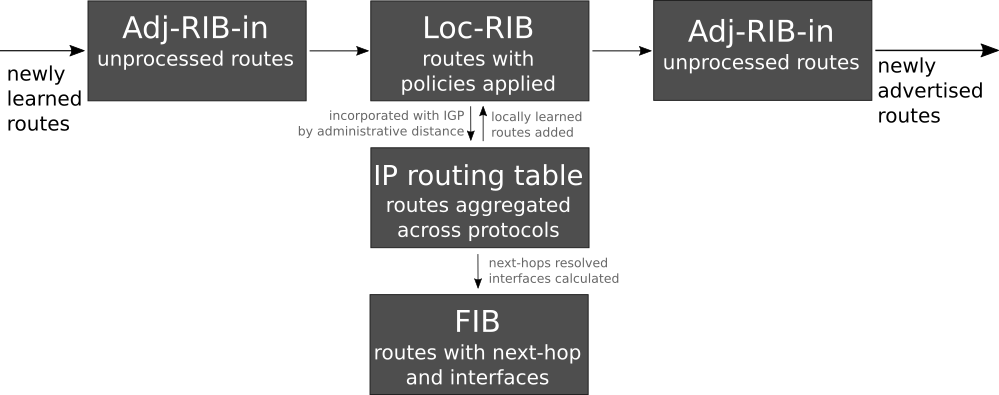
\includegraphics[scale=0.5]{img/bgp-update.png}
	\caption{BGP update process (reproduced from \cite{thousandeyes})}
	\label{fig:bgp-update}
\end{figure}

%Network reachability can be seen from two perspectives: control and data planes. Control plane focuses on building the topology as the router sees based on the routing protocol used. This information is available in router's Routing Information Base (RIB) and/or Label Information Base (LIB). Data plane, or forwarding plane, is the actual paths traversed by data packets from the users. RIB within a BGP speaker consists of three distinct things (Figure \ref{fig:bgp-update}): \texttt{Adj-RIBs-In} (unprocessed routing information learned from inbound Update messages received from other BGP speakers), \texttt{Loc-RIB} (local routing information the BGP speaker selected by applying its local policies to the routing information contained in \texttt{Adj-RIBs-In}), and \texttt{Adj-RIBs-Out} (stores information the local BGP speaker selected for advertisement to its peers)


An anycast service, which is essentially a subset of the Internet itself, is identified at network level through its announced prefixes. The anycast prefixes is part of BGP's network reachability information. To understand and analyze how the anycast catchment works at global Internet, the routing protocol running it--\textit{i.e}., BGP--should be used as the reference. However, BGP is a complex protocol, especially due to the presence of different routing policies implemented by participating organizations. One router may have different BGP route toward a specific destination compared to others, and each router has limited view of the Internet topology. Therefore, gaining knowledge of global Internet only from a single BGP router is definitely not sufficient. 

There are three methods available to get BGP routing information from multiple routers: \textit{(i)} using looking glass, \textit{(ii)} collecting BGP routing information by establishing a BGP peering session with routers using collectors, and \textit{(iii)} using BGP monitoring protocol such as BMP. The summary of these methods including well-known monitoring projects using it is presented in Table \ref{table:ch02:monitoring-methods}.

\textit{Looking glass} is a web-based application managed by operators to provide a view into the BGP routing tables of their BGP routers. It is basically an interface to execute limited range of commands inside the routers. It provides real-time information of the BGP state of a router with no possibility to access historical data. Therefore, looking glass is more appropriate for troubleshooting purposes.

%To perform large-scale BGP monitoring, BGP routing information from wide-range locations around the world needs to be collected. Some operators make BGP routing information from their routers available for monitoring purposes. These participating routers act as the probes for BGP measurement at control-plane level. 


%%%%%%%%%%%%%%%%
% sideways table
%%%%%%%%%%%%%%%%
\begin{sidewaystable}
	\centering
	\scriptsize
	\begin{tabular}{C{2cm} C{1cm} C{2.5cm} C{2cm} C{2.2cm} C{2.5cm} C{2.4cm} C{1cm} C{1cm} C{2cm}}
		\hline
		& \textbf{Start} & \textbf{Managing Organization} & \textbf{Collecting Method} & \textbf{Data Accessibility} & \textbf{Collector Locations} & \textbf{Dump Frequency} & \textbf{Historical} & \textbf{(Near) Real-Time} & \textbf{Note} \\
		\hline\hline
		Looking glass & - & Network providers & accessing router's RIB & web interface & - & - & \xmark & \cmark & real-time BGP state\\ \hline
		RIS \cite{ripe-ncc-ris}& 2001 & RIPE NCC & route collectors & MRT file, REST API & Europe, USA, Brazil, Japan, South Africa & RIB 8 hours, Update 5 min. &\cmark & \xmark & REST API via RIPEStat \\ 
		\hline
		RouteViews \cite{route-views} & 1997 & University of Oregon & route collectors & MRT file, XML stream & USA, UK, Serbia, Kenya, South Africa, Australia, Nepal, Japan, Brazil & RIB 2 hours, Update 15 min. &\cmark & \cmark & live stream is accessed using BGPMon \\ 
		\hline
		BGPMon \cite{bgpmon} & 2008 & Colorado State University & route collectors & XML stream & uses RouteViews collectors & - &\cmark & \cmark & archives accessed in MRT and bgpdump formats \\ 
		\hline 
		PCH \cite{pch} & 2010 & PCH & route collectors & MRT file, routing table overview & 100+ IXPs (details not available) & routing table snapshot daily, Update 1 min. &\cmark & \xmark & VPs are only PCH peers\\ 
		\hline
		Caida OpenBMP \cite{caida-bmp} & June 2016 & Caida \& RouteViews & BMP & Stream & uses RouteViews collectors  & RIB 1 hour, Update 1 min. &\cmark & \cmark & Still in experimental phase \\ 
		\hline
	\end{tabular}
	\caption{BGP monitoring methods}
	\label{table:ch02:monitoring-methods}
\end{sidewaystable}

The second method is by deploying BGP route collectors at various Internet exchange points (IXP) in the world. Route collector, simply referred as \textit{collector}, is a host running a collector processes (such as Quagga\footnote{\url{http://www.nongnu.org/quagga/}}) which emulates a router and establishes BGP peering sessions with one or more participating routers (referred as \textit{peers}). Each peer sends BGP Update messages to the collector each time the \texttt{Adj-RIB-out} changes, which reflecting changes to its \texttt{Loc-RIB}. For each peer, the collector maintains \texttt{adj-RIB-out} table built based on BGP Updates received. The collector periodically dumps the maintained \texttt{Adj-RIB-out} (\textit{RIB dump}) and the BGP Update messages (\textit{Update dump}) received from all of its peers since the last dump. Typically, the dump frequencies are few hours for RIB and few minutes for Updates (see Table \ref{table:ch02:monitoring-methods}). This data dump is then archived in MRT Routing Information Export \cite{rfc6396} format. 

There are two well-known global monitoring projects that use this method in large scale, namely RIPE RIS \cite{ripe-ncc-ris} and RouteViews \cite{route-views}. Both projects have been starting collecting BGP routing information from various locations and peers since the end of 1990s and make the archives available for public access\footnote{\url{http://archive.routeviews.org/}}\footnote{\url{https://www.ripe.net/analyse/internet-measurements/routing-information-service-ris/ris-raw-data}}. In fact, both repositories become the main data sources used by researchers to study various subjects, such as routing policies, Internet topologies, security, and so on. The main issue with them is their file-based distribution system and the delay due to dump interval to make the data available. To analyze a certain prefix, for example, user is required to download the dump file of time interval in interest (can be very large in size) which contains data of other prefixes as well. Performing analysis of wide-range time period would require huge amount of storage and bandwidth to download the data. Fortunately, RIPE NCC as the operator of RIS develop RIPEStat \cite{ripestat}, a web-based interface that provides access to any specific resources contained in RIS archives through its REST API. It allows user to access specific routing resource data (\textit{e.g.}, prefix, ASN) in a fast and convenient way.

Other similar projects also exist. Firstly, PCH \cite{pch} provides their BGP routing data accessible for public as well. However, instead of providing the RIB dump, they only provide snapshot of BGP routing table overview from the output command of '\texttt{show ip bgp}'. Furthermore, judging from its dump size that relatively small compared to RIS or RouteViews, we believe that its route collectors only gather information from PCH peers (not from participating organizations such as RIS or RouteViews). Second project is BGPMon \cite{bgpmon}, a distributed BGP monitoring system that provides real-time data stream in XML format for both BGP updates and RIB snapshot. It uses streamlined collectors that allows it to be more scalable on handling large number of peers. Initially, BGPMon used its own infrastructure to perform measurement. Today, it is used by RouteViews to replace Quagga as the collectors and allows RouteViews to provide live feeds. Unfortunately, BGPMon does not provide historical data access in the same way as its live stream. It stores BGP data in MRT and bgpdump formats hence retains the same issue of file-based distribution.

There are limitations with the use of BGP route information from collectors \cite{6027863,Gregori:2012:IAG:2398776.2398803}:
\begin{enumerate}[noitemsep,nolistsep]
	\item The type of information that can be collected is not always the same. Most updates from collectors' peers are \textit{full-feed} (contains the entire \texttt{Loc-RIB}). However, some updates are \textit{partial-feeds} (only a subset of its \texttt{Loc-RIB}) which may go through a filtering process before being sent to the collectors.
	\item The collector can only see what the connected router advertises. It cannot access what BGP updates a peer receives from its neighbors (peers of a peer). To get all routes, the only way is to examine the BGP \texttt{Adj-RIB-In} for each peer.
	\item some ASes are very large geographically, thus the view in each geographical region might be different for each router in that AS.
	\item The number of collectors available are quite limited, and its placement is geographically and topologically biased. The first bias especially happens in RIS, where most of its collectors reside in Europe. Second bias comes from the fact that the collectors receive data from volunteer networks that mostly are large top-tier ISPs. Therefore, many peer-to-peer connections that may be established among ASes at the Internet edges may not detected. The number of ASes that feeding the collectors are also quite small compared to the total advertised ASes on the Internet. Thus, it results in extremely narrow view of the Internet.
	\item The connections between collectors and routers are not reliable all the time. Data loss might occur anytime.
\end{enumerate}

% more about BGPMon

The third method is an attempt to improve some shortcomings above using \textit{BGP Monitoring Protocol} (BMP) \cite{ietf-bmp}. BMP is used to monitor BGP sessions, and the primary improvement over traditional BGP peering method is the capability to access \texttt{adj-RIB-in} to get complete dump of the routes received by a peer (including routes from peers of a peer). Instead of using collector, the participating peers connects to a management station, sends initial dump of all routes for those peers. As peers advertise or withdraw routes, additional updates are sent to the management station. Thus, user is not required to wait until the data dump available. OpenBMP \cite{openbmp} is an open-source implementation of BMP and supported by the latest Cisco and Juniper's OS. It allows to periodically access the \texttt{adj-RIB-in} of a router or to monitor its BGP peering sessions. 

Despite of its promising improvement, unfortunately there is no large-scale project yet that provide their BMP data publicly as RouteViews or RIS do. An experimental project conducted by Caida and RouteViews \cite{caida-bmp} to use OpenBMP on RouteViews collectors is underway to allow real-time and historical data access, which might be available for public in the near future. Therefore, despite of its imperfectness, RIS and RouteViews still provide the largest usable BGP routing datasets.

%\textbf{Read "Determining the Cause and Frequency of Routing Instability with Anycast". They use BGP data as well.}

\section{Anycast Visualization}
\label{ch02:visualization}
BGP route visualization belongs to the domain of graph drawing, which follows theory rules covered by graph theory. It is a visual representation of the vertices (link between ASes) and edges (ASes). Control-plane Anycast visualization itself can be performed using typical methods for BGP visualization. 

There are several related works on visualizing BGP topology. Since 2000, CAIDA has generated \textit{AS core graphs} (also referred as AS-level Internet graphs) representing a macroscopic snapshot of IPv4 and IPv6 Internet topology samples in order to visualize the shifting topology of the Internet over time, both for IPv4 and IPv6 \cite{caida-vis}. It ranks ASes based on their transit degree; the higher the degree the more centered is the AS placement in the graph. Inspired by CAIDA's work, APNIC developed VizAS \cite{vizas} to provide visualization of the BGP peering relationships within a single economy (e.g., a country). It shows two side-by-side IPv4 and IPv6 charts representing the visible autonomous network in the selected economy.

BGPlay \cite{bgplay} is a Java-based tool which displays animated graphs of the routing activity of a certain prefix within a specified interval to visualize the behavior and instabilities of of Internet routing at the AS level. It is fed using relevant BGP update messages for the specified time interval. BGPlay was used by Karrenberg \cite{karrenberg2005anycast} to visualize path changes between instances and probes in his study. To improve its portability, there is a work to implement BGPlay in pure JavaScript, called BGPlay.js \cite{bgplay.js}, which uses routing data in a specified JSON format. It is currently being used in RIPEstat \cite{ripestat}. 

%AUTOMATTIC, which hosts \texttt{wordpress.com},  provides visualization of their global anycast network at \cite{ac-map}. They develop Netflow-based monitoring system with one of its capabilities is to identify non-optimal anycast networks\footnote{\url{https://developer.wordpress.com/2016/02/08/open-source-netflow-with-elastic-logstash-kibana/}}.

\begin{figure}[!ht]
	\begin{subfigure}[b]{0.5\linewidth}
		\centering
		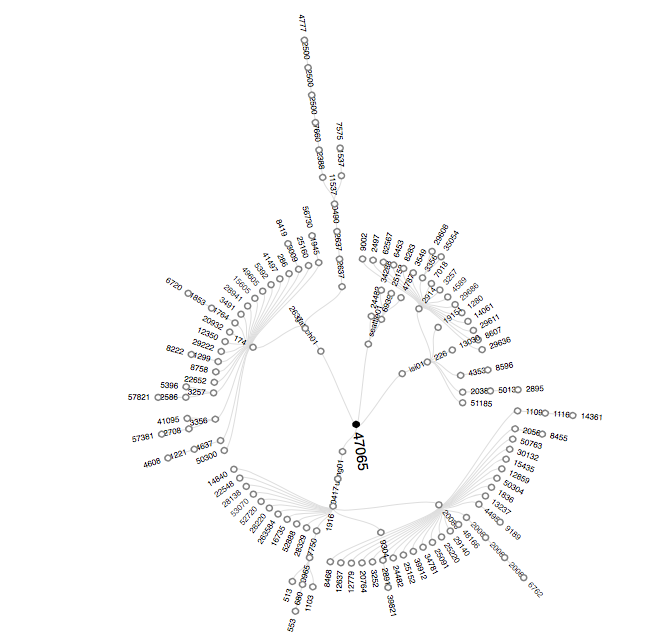
\includegraphics[width=\linewidth]{img/beforeAmestC.png}
		\caption{Control plane - before}
		\label{fig:ricardo-control-before}
	\end{subfigure}
	\begin{subfigure}[b]{0.5\linewidth}
		\centering
		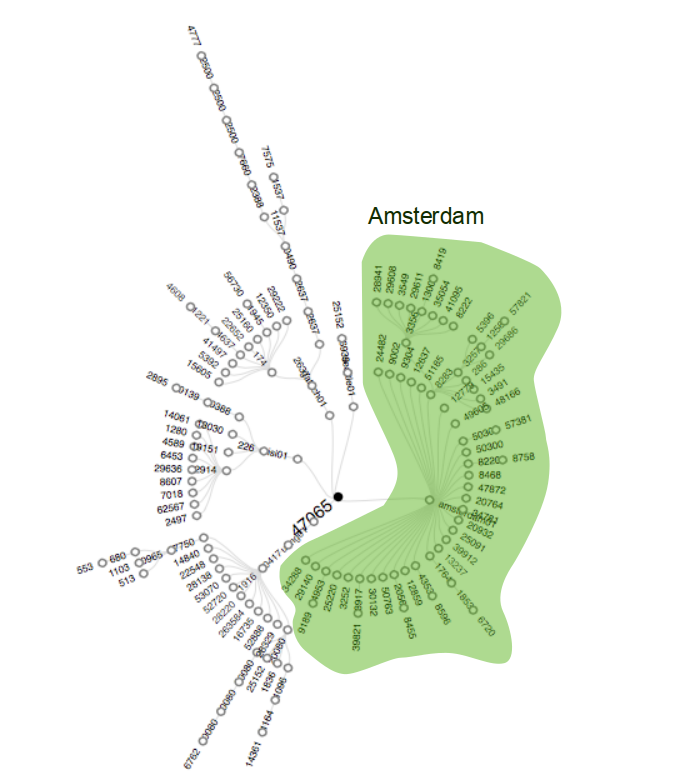
\includegraphics[width=\linewidth]{img/afterAmestC.png}
		\caption{Control plane - after}
		\label{fig:ricardo-control-after}
	\end{subfigure}
	\caption{Visualization of routing impact of adding or removing anycast instances, copied from \cite{github-anycast}}
	\label{fig:ch02:ricardo}		
\end{figure}

Specific to anycast visualization, the authors of \cite{github-anycast} proposed visualization tool for IP anycast to understand routing impact of adding or removing instances. Since BGP paths consist of a number of AS hops, it would be easier to understand if ASes with the same hop degree relative to the measured AS are grouped together. Thus, they use radial tree graph based on the Reingold-Tilford algorithm \cite{1702828} for efficient, tidy arrangement of layered nodes. They use PEERING platform \cite{peering} as the anycast testbed consisting of 7 instances spread in USA, Brazil, and the Netherlands. They use a subset of RIPE Atlas probes that periodically run \texttt{traceroute} towards PEERING. The BGP routing data is collected from both \texttt{traceroute} and RIS collectors. The tool separates the view into two segments: control and data planes. Control plane visualization is used to see the changes in BGP routes when there is a change (withdrawal or announcement) of an instance. The data is taken from RIPE RRC. In order to quantify changes take place in data plane, a periodic traceroute measurements are performed using RIPE Atlas probes. The result of their visualization for control plane is presented in Figure \ref{fig:ch02:ricardo}. It shows the anycast catchment areas before and after the instance announcement. The ASes are arranged in a hierarchy based on the degree towards the origin AS.  

To summarize, CAIDA's graph and VizAS are impressive. They are intended to visualize high-level overview of the topology by focusing more on who are the big players in the networks. Since the diameter of the outer circle is fixed, as the networks become larger with huge numbers of edge ASes then the graph becomes difficult to read due to denser outer circle. BGPlay excels at visualizing AS-level network changes over a period of time. As it visualizes every BGP Update message events, it provides very detailed information. Thus, BGPlay is more suitable as troubleshooting tool. Result from \cite{github-anycast} is the closest to the requirement of this work. Improvements can be made, especially in the interactivity part.

\section{Concluding Remarks}
\label{ch02:concluding}
%\texttt{Traceroute} and BGP routing information are the two methods used in the literature in Section \ref{ch02:measuring-anycast} to reveal anycast catchment areas. Despite of its simplicity and finer granularity, \texttt{traceroute} suffers from ICMP filtering often implemented along the path. On the other hand, BGP routing data provides high-level view of connectivity, but reveals end-to-end AS-level paths. For this study, using BGP routing data is more appropriate as we need broad view of the networks to understand the catchment areas. There are several methods to obtain BGP routing data, as listed in Table \ref{table:ch02:monitoring-methods}. As we need to study the catchment areas from the beginning of Root Servers' dual-stacked operation, the historical data access is required. The use of BMP is quite promising, due to more complete results offered. However, the large-scale project we know is running it is still in experimental phase and just started recently. Thus, it leaves us with the route collector-based projects as the data repository.
\texttt{Traceroute} and BGP routing information are the two methods used by literature to reveal anycast catchment areas. Despite of its simplicity and finer granularity, \texttt{traceroute} suffers from ICMP filtering often implemented along the path. On the other hand, BGP routing data provides high-level view of connectivity, but reveals end-to-end AS-level paths. For this study, using BGP routing data is more appropriate as we need broad view of the networks to understand the catchment areas. In order to obtain historical BGP routing data, using public data from measurement projects such as RIS and RouteViews is preferred over other approaches. Finally, to visualize comparison of IPv4 and IPv6  anycast catchment area, work in \cite{github-anycast} is the closest to this work, and thus it can be developed further to fit our requirements and to include interactivity features.
